\begin{sidewaysfigure}[h]
\centering
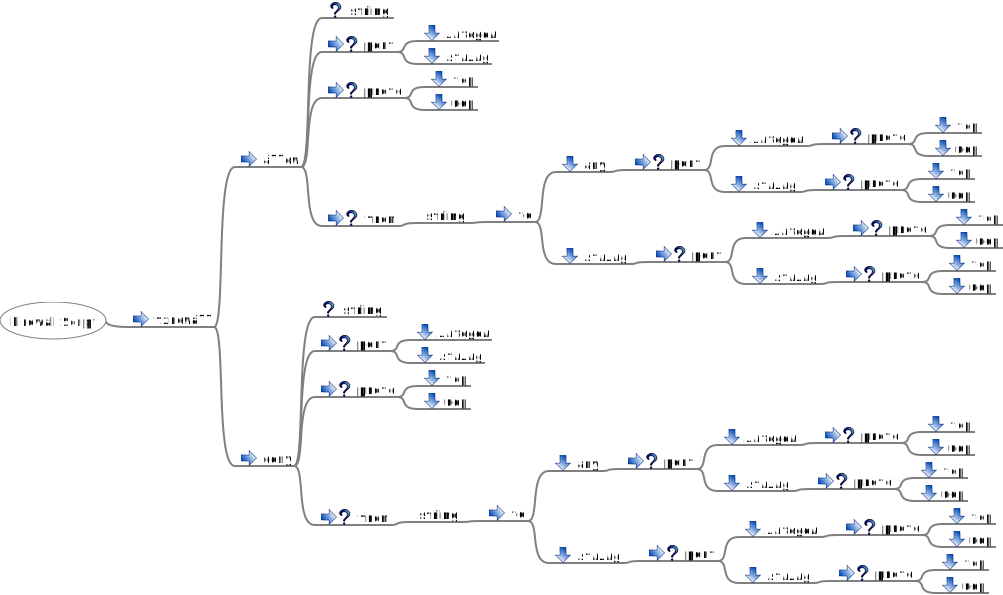
\includegraphics[width=1.0\textheight]{firewall_service_script}
\label{fig:firewall_script_statements}
\caption{Firewall Script Statements}
\end{sidewaysfigure}

\begin{lstlisting}[style=Java,label=lst:firewall_allow_script,caption=Firewall Allow Rules Script]
firewall {

    // allow from all ports, all addresses to all ports to all addresses
    allow

    // allow port 22/tcp/udp on the host to anywhere
    allow port: 22

    // allow port 22/tcp on the host to anywhere
    allow port: 22, proto: tcp

    // allow port 22/udp on the host to anywhere
    allow port: 22, proto: udp

    // allow port 22/tcp/udp on the host to anywhere
    allow port: "ssh"

    // allow from anywhere to anywhere on the host
    allow from: any to any

    // allow from anywhere port 22 to anywhere port 23 on the host
    allow from: any, port: 22 to any, port: 23

    // allow from anywhere port 22 to anywhere port 23 on the host
    allow from: any, port: "ssh" to any, port: "www"

    // allow from 192.168.0.1 to anywhere port 23 on the host
    allow from: "192.168.0.1" to any, port: 23

    // allow from 192.168.0.1 port 22 to 127.0.0.1 port 23 on the host
    allow from: "192.168.0.1", port: 22 to "127.0.0.1", port: 23

    // allow from 192.168.0.1 port 22/tcp to 127.0.0.1 port 23/udp on the host
    allow from: "192.168.0.1", port: 22, proto: tcp to "127.0.0.1", port: 23, proto: udp

    // allow from 192.168.0.1 port 22/tcp to 127.0.0.1 port 23/udp on the host
    allow from: "192.168.0.1", port: "ssh", proto: tcp to "127.0.0.1", port: 23, proto: udp

    // allow from 192.168.0.1 port ssh/tcp to 127.0.0.1 port http/udp on the host
    allow from: "192.168.0.1", port: "ssh", proto: tcp to "127.0.0.1", port: "http", proto: udp

    // allow from 192.168.0.1 port 22/udp to 127.0.0.1 port 23/tcp on the host
    allow from: "192.168.0.1", port: 22, proto: udp to "127.0.0.1", port: 23, proto: tcp

}
\end{lstlisting}

\pagebreak

\begin{lstlisting}[style=Java,label=lst:firewall_deny_script,caption=Firewall Deny Rules Script]
firewall {

    // deny from all ports, all addresses to all ports to all addresses
    deny

    // deny port 22/tcp/udp on the host to anywhere
    deny port: 22

    // deny port 22/tcp on the host to anywhere
    deny port: 22, proto: tcp

    // deny port 22/udp on the host to anywhere
    deny port: 22, proto: udp

    // deny port 22/tcp/udp on the host to anywhere
    deny port: "ssh"

    // deny from anywhere to anywhere on the host
    deny from: any to any

    // deny from anywhere port 22 to anywhere port 23 on the host
    deny from: any, port: 22 to any, port: 23

    // deny from anywhere port 22 to anywhere port 23 on the host
    deny from: any, port: "ssh" to any, port: "www"

    // deny from 192.168.0.1 to anywhere port 23 on the host
    deny from: "192.168.0.1" to any, port: 23

    // deny from 192.168.0.1 port 22 to 127.0.0.1 port 23 on the host
    deny from: "192.168.0.1", port: 22 to "127.0.0.1", port: 23

    // deny from 192.168.0.1 port 22/tcp to 127.0.0.1 port 23/udp on the host
    deny from: "192.168.0.1", port: 22, proto: tcp to "127.0.0.1", port: 23, proto: udp

    // deny from 192.168.0.1 port 22/tcp to 127.0.0.1 port 23/udp on the host
    deny from: "192.168.0.1", port: "ssh", proto: tcp to "127.0.0.1", port: 23, proto: udp

    // deny from 192.168.0.1 port ssh/tcp to 127.0.0.1 port http/udp on the host
    deny from: "192.168.0.1", port: "ssh", proto: tcp to "127.0.0.1", port: "http", proto: udp

    // deny from 192.168.0.1 port 22/udp to 127.0.0.1 port 23/tcp on the host
    deny from: "192.168.0.1", port: 22, proto: udp to "127.0.0.1", port: 23, proto: tcp

}
\end{lstlisting}

\pagebreak

\begin{lstlisting}[style=Java,label=lst:firewall_ubuntu_profile,caption=Firewall Example Ubuntu Profile]
profile "ubuntu_10_04", {
    system {
        install_command "/usr/bin/aptitude update && /usr/bin/aptitude install"
    }
    firewall {
        service "ufw"
        ufw_command "/usr/sbin/ufw"
    }
}
\end{lstlisting}

\begin{longtable}{lp{0.5\textwidth}}
\multicolumn{2}{l}{Commands Properties} \\*
\toprule
\endfirsthead
\endhead
\caption{UFW Ubuntu 10.04 Properties}
\label{tbl:firewall_ufw_ubuntu_10_04_properties}
\endlastfoot
%
install\_command &
\code{/usr/bin/aptitude update \&\& /usr/bin/aptitude install} \\
%
ufw\_command &
\code{/usr/sbin/ufw} \\
%
\toprule
%
\multicolumn{2}{l}{Other Properties} \\*
\toprule
%
packages &
\code{ufw} \\
%
\end{longtable}

